\section{Syntax directed typing}

\subsection{Constraint language}

\newcommand\A{\mathcal A}
\newcommand\SC{\mathcal S}

Let us note $\A$ our constraint system. The full grammar of constraints is
given in \cref{grammar:constraint}.
$\A$ is defined as the smallest cylindric term constraint system that
satisfies the axiom shown in \cref{rules:entail}.
We follows the traditional HM(X) formulation
with conjunctions, projections and type inequalities.
The new element specific to our approach are kind inequalities.
Entailment is noted $\entail{C}{D}$, where $D$ is a consequence of the
constraints $C$.
We say that $C$ and $D$ are equivalent, noted $C \equivC D$,
when $\entail{C}{D}$ and $\entail{D}{C}$.
\TODO{Give the cylindric properties ?}

\begin{figure}[tp]
  \centering
  \begin{align*}
    C &::= \Cleq{\tau_1}{\tau_2}
        \mid \Cleq{k_1}{k_2}
        \mid C_1 \Cand C_2
        \mid \Cproj{\tvar}{C}
        \mid \Cproj{\kvar}{C}
  \end{align*}
  \caption{The constraint language}
  \label{grammar:constraint}
\end{figure}

\begin{figure*}[tp]
  \begin{minipage}{0.65\linewidth}
  \begin{mathpar}
    \inferrule[Lat-UAL]{}{\kun \lk \kaff \lk \klin}
    \and
    \inferrule[Lat-Level]{\mul \lk \mul' \and n \lk n'}{\mul_n \lk_\Lat \mul'_{n'}}
  \end{mathpar}
\end{minipage}~
\begin{minipage}{0.2\linewidth}
  \centering
  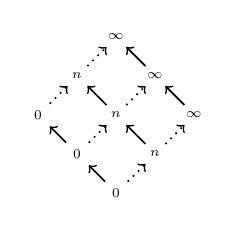
\begin{tikzpicture}
    [->,auto,semithick, every node/.style={scale=0.7}]
    \node(U) {$\kun_0$} ;
    \node(A) [above left of=U] {$\kaff_0$} ;
    \node(L) [above left of=A] {$\klin_0$} ;
    \node(Un) [above right of=U] {$\kun_n$} ;
    \node(An) [above left of=Un] {$\kaff_n$} ;
    \node(Ln) [above left of=An] {$\klin_n$} ;
    \node(Uinf) [above right of=Un] {$\kun_\infty$} ;
    \node(Ainf) [above left of=Uinf] {$\kaff_\infty$} ;
    \node(Linf) [above left of=Ainf] {$\klin_\infty$} ;
    \path
    (U) edge (A)
    (A) edge (L)
    (Un) edge (An)
    (An) edge (Ln)
    (Uinf) edge (Ainf)
    (Ainf) edge (Linf)
    ;
    \path[dotted]
    (U) edge (Un)
    (A) edge (An)
    (L) edge (Ln)
    (Un) edge (Uinf)
    (An) edge (Ainf)
    (Ln) edge (Linf)
    ;
  \end{tikzpicture}
\end{minipage}

%%% Local Variables:
%%% mode: latex
%%% TeX-master: "../main"
%%% End:

  \caption{Lattice inequalities -- $k \lk_\Lat k'$}
  \begin{mathpar}
  \inferrule
  {}{ \entail{}{\Cleq{\kvar}{\kaff}} }
  \and
  \inferrule
  {}{ \entail{}{\Cleq{\kun}{\kvar}} }
  \and
  \inferrule
  {}{ \entail{}{\Cleq{\kvar}{\kvar}} }
  \and
  % \inferrule
  % {\Cleq{k}{k'} \in C}{ \entail{C}{\Cleq{k}{k'}} }
  % \and
  % \inferrule
  % { \entail{C}{\Cleq{x_1}{x}}\\
  %   \entail{C}{\Cleq{x}{x_2}}
  % }
  % { \entail{C}{\Cleq{x_1}{x_2}} }
  % \and
  % \inferrule
  % { \entail{C}{D} }
  % { \entail{C}{\Cproj{x}{D}} }
  % \\
  \inferrule
  { \entail{C}{\Cleq{\tau'_1}{\tau_1}}\\
    \entail{C}{\Cleq{\tau_2}{\tau'_2}}\\
    \entail{C}{\Cleq{k}{k'}}
  }
  { \entail{C}{\Cleq{\tau_1\tarr{k}\tau_2}{\tau'_1\tarr{k'}\tau'_2}} }
  \and
  \inferrule
  { \forall i,\ \entail{C}{\Cleq{\tau_i}{\tau_i}}\\
  }
  { \entail{C}{\Cleq{\tapp{t}{(\tau_i)}}{\tapp{t}{(\tau'_i)}}} }
  \and
  
  % \and
  % \inferrule
  % { \entail{C}{\Cleq{k}{k'}} \\
  %   \entail{C}{\Cleq{k'}{k}} }
  % { \entail{C}{\Ceq{k}{k'}} }
  % \and
  % \inferrule
  % { \entail{C}{\Cleq{k}{k'}} }
  % { \entail{C}{\Ckind{\tau_0\tarr{k}\tau_1}}{k'}}
  % \and
  % \text{Completion to form a cylindric constraint system.}
\end{mathpar}

%%% Local Variables:
%%% mode: latex
%%% TeX-master: "../main"
%%% End:

  \caption{Base entailment rules -- $\entail{C}{D}$ }
  \label{rules:entail}
\end{figure*}


We note $\SC$ the set of solved forms
which can be used inside type and kind schemes.
We define $\SC$ as $\A$ quotiented by the relation $\equivC$.
%
We consider the existence of a function $\operatorname{normalize}$ which takes
a constraint in $\A$ and a substitution $\psi$ and returns a constraint
in solved form $C' \in \SC$,
and an updated substitution. We detail the implementation
of the normalization function in \cref{sec:normalize}

% $\mathcal S$ is composed only of kind
% inequalities \emph{over variables}. For convenience, if $C\in\mathcal S$, we
% note $C$ as a list of kind inequalities: $\Cleq{\kvar_i}{\kvar_{i'}}^n$.
% \TODO{Extend the properties of solved forms}

\subsection{Kinding}

We note $\inferSK{C}{\E}{\tau}{k}$
when $\tau$ has kind $k$ in environment $\E$ under constraints $C$.
The rules are shown in \cref{rules:sd-kinding}.
Kinds and types follow a small calculus with variables ($\tvar$,\dots),
functions (type constructors $\T{t}$), application ($\tapp{t}{\Multi{\tau}}$)
and primitives such as types for arrows ($\tau\tarr{k}\tau'$) and
borrows ($\borrowty{k}{\tau}$).
Kind checking can thus be done in a fairly straightforward, syntax-directed
fashion by simply following
the syntax of the types. Kind arrows can only appear when looking
up the kind scheme of a type constructor $\T t$. Kind arrows are forbidden
in any other contexts.


\begin{figure}[ht]
  \centering
  \begin{mathpar}
  \inferrule[KVar]
  { \bvar{\tvar}{k} \in \E }
  { \inferSK{C}{\E}{\tvar}{k}
  }
  \and
  \inferrule[KPair]
  { \forall i \quad
    \inferSK{C}{\E}{\tau_i}{k_i} \quad
    \inferSS{C}{\E}{k_i}{k}
  }
  { \inferSK{C}{\E}{\tyPair{\tau_1}{\tau_2}}{k} }
  \and
  \inferrule[KApp]
  { \bvar{\T{\tcon}}{
      \forall \Multi[i]\kvar.\ \qual{D}{(\Multi[j]{k'}) \karr k'}}
    \in \E \\
    \unif = \subst{\Multi[i]\kvar}{\Multi[i]k}{} \\
    \entail C {\unif D} \\
    \forall j\quad
    \inferSK{C}{\E}{\tau_j}{k_j}\quad
    \inferSS{C}{\E}{k_j}{\unif{k'_j}}
  }
  { \inferSK{C}{\E}{\tapp{\tcon}{\Multi[j]{\tau}}}{\unif{k'}} }
  \and
  \inferrule[KBorrow]
  {}{ \inferSK{C}{\E}{\borrowty{k}{\tau}}{k}}
  \and
  \inferrule[KArr]
  {}
  { \inferSK{C}{\E}{\tau_1 \tarr{k} \tau_2}{k} }
\end{mathpar}


%%% Local Variables:
%%% mode: latex
%%% TeX-master: "../main"
%%% End:

  \caption{Syntax-directed kinding rule --
    $\inferSK{C}{\E}{\tau}{k}$}
  \label{rules:sd-kinding}
\end{figure}

\subsection{Environments}

\begin{figure}[tp]
  \begin{mathpar}
  \inferrule[ESplit-Empty]{}{
    \bsplit{\Cempty}\Eempty\Eempty\Eempty
  }

  \inferrule[ESplit-Nonempty]{
    \bsplit{C_1}{\E}{\E_1}{\E_2} \\
    \bsplit{C_2}{b}{b_1}{b_2}
  }{
    \bsplit{C_1\Cand C_2}{\E;b}{\E_1;b_1}{\E_2;b_2}
  }

  \inferrule[ESplit-Check]{
    \bsplit{D}{\E}{\E_1}{\E_2} \\
    \entail{C}{D}
  }{
    \lsplit{C}{\E}{\E_1}{\E_2}
  }
\end{mathpar}
\hrulefill
\begin{mathpar}
  \inferrule[BSplit-Both]{}{
    \bsplit {\Cleq{\schm}{\kun_\infty}}
    {\bvar{x}{\schm}} {\bvar{x}{\schm}} {\bvar{x}{\schm}}
  }

  \inferrule[BSplit-Left]{}{
    \bsplit {\Cempty} {\bvar{x}{\schm}} {\bvar{x}{\schm}} {\bnone}
  }

  \inferrule[BSplit-Right]{}{
    \bsplit {\Cempty} {\bvar{x}{\schm}} {\bnone} {\bvar{x}{\schm}}
  }

  \inferrule[BSplit-Imm-Borrow]{}{
    \bsplit {\Cempty}
    {\bvar{\borrow[\IBORROW]{x}}{\schm}}
    {\bvar{\borrow[\IBORROW]{x}}{\schm}}{\bvar{\borrow[\IBORROW]{x}}{\schm}}
  }

  \inferrule[BSplit-To-Borrow]{}{
    \bsplit {\Cempty}{\bvar x \schm}{\svar x \schm^n}{\bvar x \schm}
  }

  \inferrule[BSplit-To-Imm]{}{
    \bsplit {\Cempty}
    {\bvar{\borrow x} \schm}{\svar[\IBORROW] x \schm^n}{\bvar{\borrow x} \schm}
  }
\end{mathpar}
%%% Local Variables:
%%% mode: latex
%%% TeX-master: "../main"
%%% End:

  \caption{Splitting --- environments $\lsplit
    C\E\E\E$; binders $\bsplit Cbbb$}
  \label{fig:sd-splitting}
\end{figure}

\begin{figure}[tp]
  \begin{mathpar}
  \inferrule[EBorrow]{
    \bregion{C_r}{}{\svar{x}{\tau}^n}{b}
  }{
    \bregion{C_r}{x}{\E;\svar{x}{\tau}^n}{\E; b}
  }

  \inferrule[EBorrow-Check]{
    \entail{C}{D}\\\\
    \bregion{D}{x}{\E;\svar{x}{\tau}^n}{\E; b}
  }{
    \lregion{C}{x}{\E;\svar{x}{\tau}^n}{\E; b}
  }
  
  \inferrule[EBorrow-Binder]{
    \BORROW\in\left\{\kun,\kaff\right\}\\
    C = (\BORROW_n\lk k) \wedge (k \lk \BORROW_\infty)
  }{
    \bregion{C}{}
    {\svar[\BORROW]{x}{\tau}^n}
    {\bvar{\borrow[\BORROW]{x}}{\borrowty[\BORROW] k{\tau}}}
  }
\end{mathpar}
%%% Local Variables:
%%% mode: latex
%%% TeX-master: "../main"
%%% End:

  \caption{Borrowing --- environments $\lsplit
    C\E\E\E$; binders $\bsplit Cbbb$}
  \label{fig:sd-borrowing}
\end{figure}

\subsection{Typing}

\begin{figure*}[tp]
  \begin{mathpar}
  \inferrule{}{ \Cleq{\Eempty}{k} \Crewrite  \Cempty}

  \inferrule{
    \Cleq\E k \Crewrite  C \\ \E \vdash \Cleq B k \Crewrite  D
  }{
    \Cleq{\E; B}{k} \Crewrite  C \Cand D
  }
  \\
  \inferrule{
    \E \vdash \Cleq \schm k \Crewrite  C
  }{ \E \vdash \Cleq{\bvar x \schm}{k} \Crewrite  C}

  \inferrule{
    \E \vdash \Cleq \schm k \Crewrite  C \\
    \Cleq{\BORROW^n} k  \Crewrite  D
  }{
    \E \vdash \Cleq{\svar x \schm^n} k \Crewrite  C \Cand D
  }
  \\
  \inferrule{}{\Cleq{\IBORROW^n} k \Crewrite  \Cleq{\kun_n} k}

  \inferrule{}{\Cleq{\MBORROW^n} k \Crewrite  \Cleq{\kaff_n} k}
  \\
  \inferrule{
    \E; \Multi{\bvar{\alpha}{k}} \vdash \Cleq\tau k \Crewrite  D
  }{
    \E \vdash \Cleq{\forall\Multi\kvar\forall\Multi{\bvar{\alpha}{k}}.(\qual{C}{\tau})}
    k \Crewrite  C \Cand D
  }

  \inferrule{}
  { \E \vdash \Cleq{ \tau_2\tarr{k'}\tau_1 } k \Crewrite  \Cleq{k'}k }

  \inferrule{
    \E(\tvar) = \kschm
  }
  { \E \vdash \Cleq{ \tvar} k \Crewrite  \Cleq\kschm k }

  \inferrule{
  }{ \E \vdash \Cleq{\tapp{t}{\Multi\tau}} k \Crewrite  ???}

  \inferrule{}{
    \E \vdash \Cleq{\borrowty {k'} {\tau}} k \Crewrite  \Cleq{k'}k
  }
\end{mathpar}

%%% Local Variables:
%%% mode: latex
%%% TeX-master: "../main"
%%% End:

  \caption{Rewriting constraints on environments and types}
  \label{fig:contraints-environments-types}
\end{figure*}
\begin{figure*}[tp]
  \begin{mathpar}
  \inferrule[Scheme]{
    \inferSK{C \Cand C_x} \E \tau {k'} \\
    \entail C {\Cleq{k'}k}
  }{
    \entail C {(\forall \kvar_i \forall (\tvar_j:k_j).\
      \qual{C_x}{\tau}) \le  k}
  }
\end{mathpar}
\hrulefill
\begin{mathpar}
  \inferrule[Var]
  { \bvar{x}{
      \forall \kvar_i \forall (\tvar_j:k_j).\ \qual{C_x}{\tau}
    }
    \in \E \\
    \unif = [\kvar_i\mapsto k_i,\tvar_j \mapsto \tau_j] \\
    \entail C {\unif(C_x)} \\
    % \addlin{
    %   \inferSK{C}{\E}{\unif \tau}{k_\tau}
    % }
  }
  { \inferS{C}{\E}{x}{\unif\tau}
  }
  \and
  \ruleSDLam
  \and
  \ruleSDApp
  \and
  \inferrule[Let]
  { \inferS{C \Cand D}{\E_1}{e_1}{\tau_1} \\
    \schm = \forall\Multi\kvar\forall\bvar{\Multi\tvar}{\Multi{
        k}}. \qual{D}{\tau_1}\\
    \{\Multi\kvar, \Multi\tvar\} = \fv{D, \tau_1} \setminus \fv{C, \E}
  \\
  \entail{C}{\exists\Multi\kvar\Multi\tvar.D} \\
    \inferS{C}{\E;\bvar{x}{\sigma}}{e_2}{\tau_2} \\
    \addlin{\lsplit{C}{\E}{\E_1}{\E_2}}\\
  }
  { \inferS{C}
    {\E}{\letin{x}{e_1}{e_2}}{\tau_2} }
  \and
  \inferrule[Pair]
  { \inferS{C}{\E_1}{e_1}{\tau_1} \\
    \inferS{C}{\E_2}{e_2}{\tau_2} \\
    \addlin{\lsplit{C}{\E}{\E_1}{\E_2}}
  }
  { \inferS{C}{\E}{\introPair{e_1}{e_2}}{\tyPair{\tau_1}{\tau_2}} }
  \and
  \inferrule[MatchPair]
  { 
    \inferS{C}{\E_1}{e_1}{\tyPair{\tau_1}{\tau'_1}} \\
    \inferS{C}
    {\E_2;\bvar{x}{\tau_1};\bvar{x'}{\tau'_1}}{e_2}{\tau_2} \\
    \addlin{\lsplit{C}{\E}{\E_1}{\E_2}}
  }
  { \inferS{C}
    {\E}{\matchin{x,x'}{e_1}{e_2}}{\tau_2} }
  \and
  %
  \inferrule[Borrow]
  { 
    \bvar{\borrow x}{\borrowty k\tau} \in \E
  }
  { \inferS{C}{\E}{\borrow{x}}{\borrowty{k}{\tau}} }
  \and
  \inferrule[Region]
  { \svar x {\tau_x} \in \E \\
    \addlin{ \bregion{C_r}{x}{\E}{\E'} }\\
    \inferS{C}{\E'}{e}{\tau} \\
    \inferSK{C}{\E}{\tau}{k_\tau}\\
    \entail C {\Cleq{k_\tau}{\klin_{n-1}}} \\
  }  { \inferS{C}{\E}{\region{x}{e}}{\tau} }
  \and
  %
  % \inferrule[Elim]
  % { \tvar,(\kvar'_i),(\tvar'_j)\text{ new}\\
  %   \bvar{K}{
  %     \forall \kvar_i \forall (\tvar_j:\kvar_j).\ \qual{C_K}{\tau_1 \tarr{}\tau_2}
  %   } \in \E\\
  %   \inferW{\Sv}{(C,\unif)}{\E}{e}{\tau} \\
  %   \unif' =
  %   \subst{\kvar_i}{\kvar'_i}{} \meet
  %   \subst{\tvar_j}{\tvar'_j}{} \meet \unif \\
  %   D =
  %   C \Cand C_K \Cand \Cleq{\tau_1}{\tvar} \Cand \Cleq{\tau}{\tau_2} \\
  %   (C,\unif) = \normalize{D}{\unif'}\\
  % }
  % { \inferW{\addlin{\Sv}}{(C,\unif|_{\fv{\E}})}{\E}{\elimK{K}{e}}
  %   {\unif\tvar} }
\end{mathpar}

% \begin{align*}
%   \Weaken(x,\Sv)
%   &\equiv \begin{cases}
%     \operatorname{kind}(x)\lk\kun &\text{if } \operatorname{kind}(x)\in\Sv\\
%     \Cempty &\text{otherwise}
%   \end{cases}\\
%   \Cleq{\Sv}{k}
%   &\equiv \bigwedge_{\kvar\in\Sv} \Cleq{\kvar}{k}
% \end{align*}

%%% Local Variables:
%%% mode: latex
%%% TeX-master: "../main"
%%% End:

  \caption{Syntax-directed typing rules}
  \label{fig:syntax-directed-typing}
\end{figure*}

%%% Local Variables:
%%% mode: latex
%%% TeX-master: "../main"
%%% End:
